\chapter{Using satellite images}\label{ch:useSat}
%
The following chapter overviews the processing of satellite images data using \texttt{MicMac} tool. The content is structured into several sections, 
\begin{itemize}
\item Section~\ref{sec:rpcBundle} regarding the processing of images delivered with the the rational polynomial coefficients (RPCs),
\item Section~\ref{sec:gridProc} regarding images that hold the GRID/RTO orientation data,
\item Section~\ref{sec:epiSatel} regarding the resampling of satellite imagery to epipolar geometry, and
\item Section~\ref{sec:sake} regarding correlation of satellite images for the purpose of change detection.
\end{itemize}
 
%
\section{With approximate sensor orientation -- RPC bundle adjustment (recommended)}\label{sec:rpcBundle}
%{\tt MicMac}
This section presents the processing chain on pushbroom sensor images when input orientation is provided in form of the RPCs. Figure~\ref{FIG:sat:func} depicts the DSM generation processing workflow. The input format of the RPCs should comply with the following: Dimap v2 (tested), DigitalGlobe (tested), IKONOS/ASCII (not fully tested). In case of IKONOS/ASCII input, the metadata -- file containing informtion about the sensor size and validity zones -- must be named \textit{Metadata.txt}. Bundle adjustment observations must include tie points and optionally may include GCP data.\par  
%
Having converted the RPC files to the {\tt MicMac}-format files (see Subsection~\ref{subsec:rpcConv}), the refinement of the orientation parameters is done within the {\tt Campari} tool (2a in Figure~\ref{FIG:sat:func}; see also Subsection~\ref{subsub:rpcCampari}). In order to validate the internal accuracy of the retrieved new orientation parameters, the user can conduct matching in the direction perpendicular to the epipolar curve with {\tt MMTestOrient}.\par 
%
If the image pair epipolar geometry is of interest, be it for external uses or to perform the matching on, the {\tt CreateEpip} tool will resample the images so that their corresponding image points are found in the same image rows.\par 
%
The dense matching is launched through the simplified {\tt Malt} tool. If matching in epipolar geometry shall be performed, use {\tt mm3d MICMAC} with a suitable XML file (see a template XML file in {\tt include/XML\_MicMac/MM-Epip.xml}).\par 
%
The reader is encouraged to follow a use case example included in Section~ \ref{sec:usecase:satel}. 

\begin{figure}[h!]
\centering 
{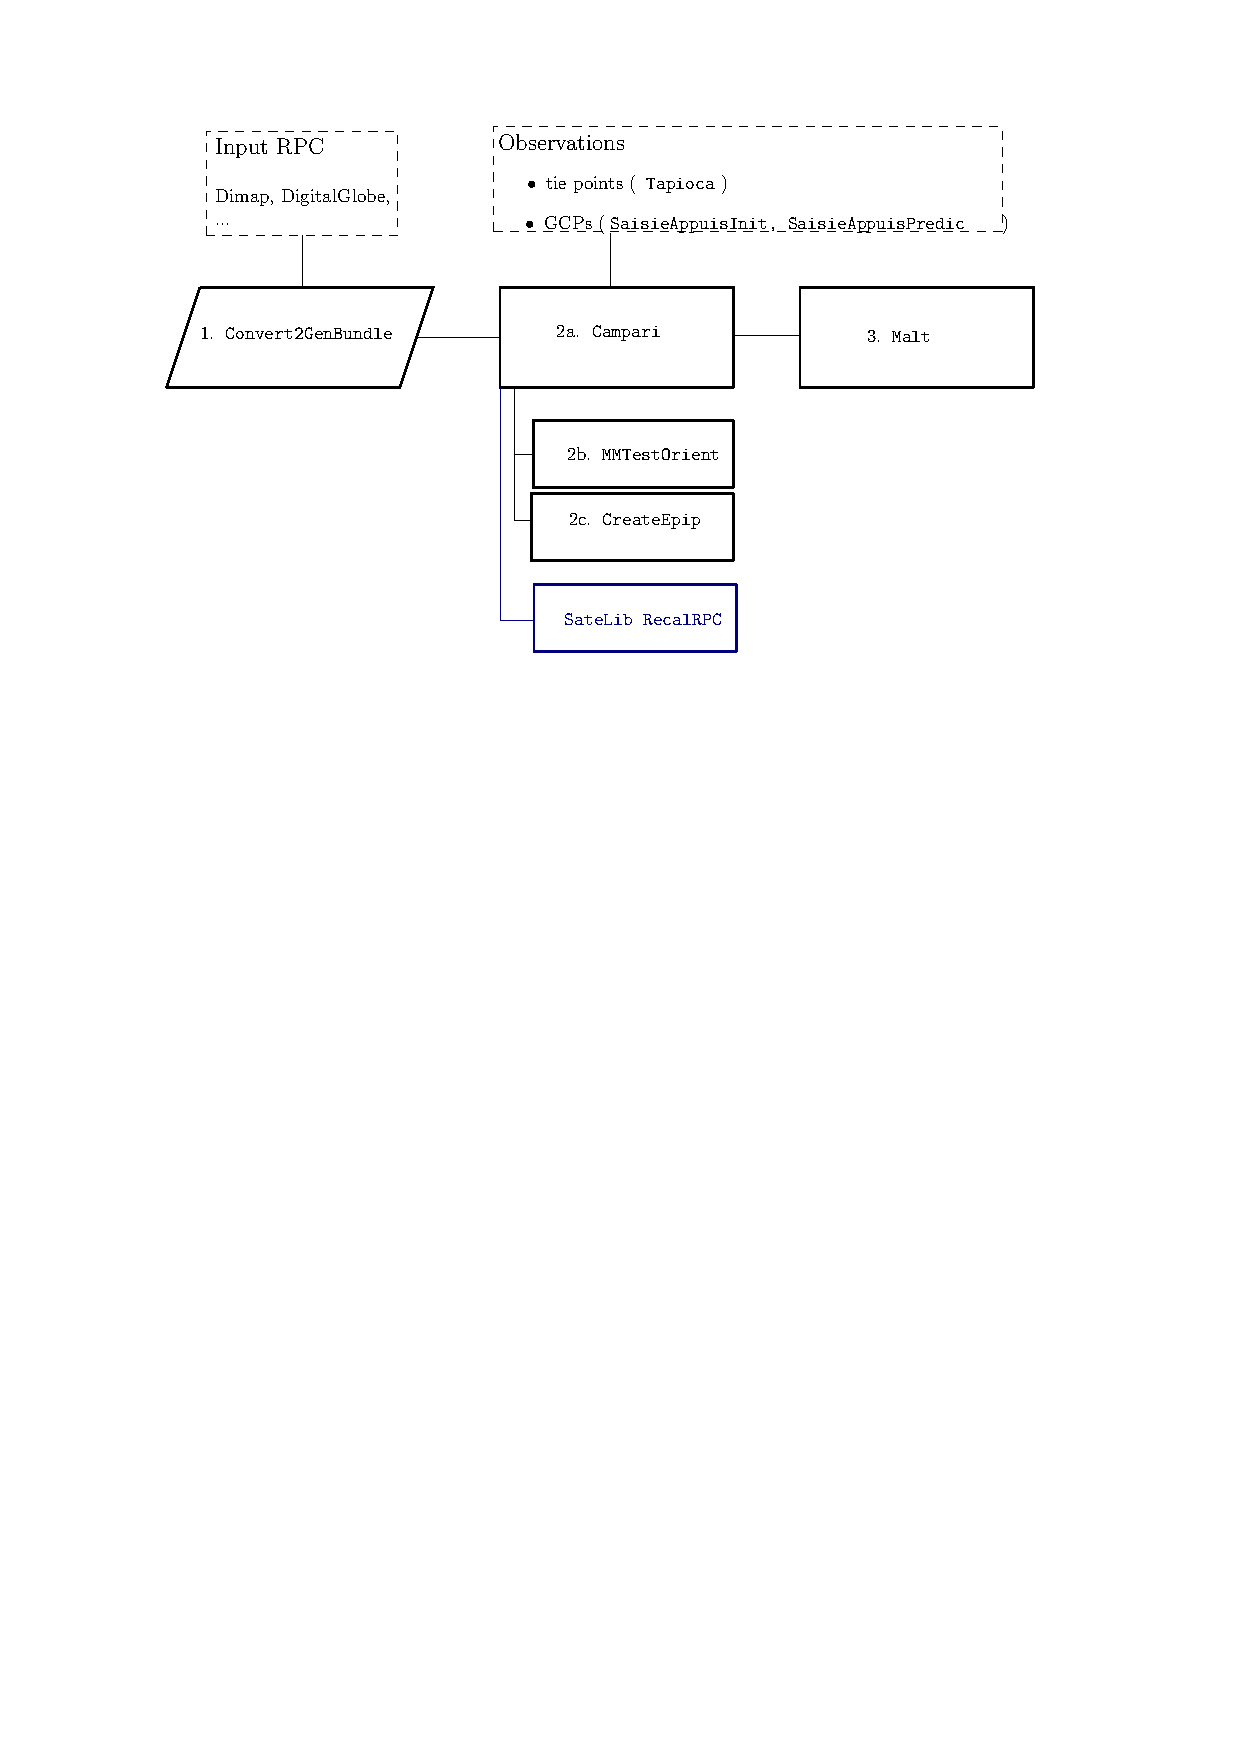
\includegraphics[width=0.88\linewidth]{FIGS/Satellites/usingSatellites.pdf}\label{FIG:sat:func}}
\caption{ Satellite images processing workflow for DSM generation. The {\tt MMTestOrient} is a supplementary operation aiming at evaluating the goodness of the orientation parameters. The {\tt CreateEpip} is obligatory only in case the user wants to perform dense matching in this geometry. {\tt{SateLib RecalRPC}} recalculates the original RPCs to include the adjusted corrections.}
\end{figure}

\subsection{ The RPC convertion to {\tt MicMac}-format files}\label{subsec:rpcConv}
The RPC orientation parameters provided by different vendors have different file formats. Due do that, prior to the actual processing {\tt MicMac} requires executing a data conversion step -- {\tt Convert2GenBundle}. As {\tt MicMac} works in uniform units, the initial RPCs defined in geodetic coordinates are recomputed in a metric coordinate system specified by the user.

\vspace{\baselineskip}
Typing {\tt mm3d Convert2GenBundle}, one gets:

\begin{verbatim}
*****************************
*  Help for Elise Arg main  *
*****************************
Mandatory unnamed args : 
  * string :: {Name of Image}
  * string :: {Name of input Orientation File}
  * string :: {Directory of output Orientation (MyDir -> Oi-MyDir)}
Named args : 
  * [Name=ChSys] string :: {Change coordinate file (MicMac XML convention)}
  * [Name=Degre] INT :: {Degre of polynomial correction (Def=2)}
\end{verbatim}

The meaning of optional args is:

\begin{itemize}
   \item {\tt ChSys}, indicates the coordinate system for the processing; the files must be edited according to the {\tt SystemeCoord} type, and contain a single {\tt BSC} (see below),
   \item {\tt Degre}, indicates the degree of the 2D polynomial adopted for orientation refinement,
\end{itemize}

Below is an example of the coordinate system file. It uses the UTM coordinate system defined over the 31. zone of the northern hemisphere, in the WGS84 datum:

\begin{verbatim}
<SystemeCoord>
     <BSC>
          <TypeCoord>eTC_Proj4</TypeCoord>
          <AuxStr>+proj=utm +zone=31 +ellps=WGS84 +datum=WGS84 +units=m +no_defs</AuxStr>
     </BSC>
</SystemeCoord>
\end{verbatim}

%* adjustment
%Campari
%MMTestOrient
%digression to Apero and parameters (cite the paper for equations)

%* matching & CO
%Malt
%CreateEpip


\section{With approximate or refined sensor orientation \\-- the GRID/RTO processing}\label{sec:gridProc}
This section presents some tools for processing satellite images that are adapted to work on the localization GRIDs. Hence, if the input orientation is known in form of rational polynomial functions, the library will need to convert it to a localization GRID, or better, switch to Section~\ref{sec:rpcBundle} to work directly on the RPCs. A sub-library for importing satellite meta-data from diverse data providers is being developed and is accessible through {\tt mm3d SateLib}.

\subsection{Pleiades-Spot or DigitalGlobe very high resolution optical satellite images}

Tools to convert RPC files into localization grids called {\tt Dimap2Grid} and {\tt DigitalGlobe2Grid} allows using VHR optical satellite images with {\tt Malt}.\\*

User has to provide:
\begin{itemize}
\item a RPC file for each image
\item cartographic step (pixels)
\item projection system
\end{itemize}

As initial localization is not always good enough to run a good correlation process, a refine step has been added to improve the grid.

\subsubsection{Image couple}

The way to get grids from an image couple is as following (example given with {\tt Dimap2Grid}, valid for {\tt DigitalGlobe2Grid}) :

\begin{itemize}
\item Dimap2Grid for each image (produces a rough grid)
\item Tapioca (generates tie-points)
\item RefineModel (computes affinity coefficients)
\item Dimap2Grid with option refineCoef (produces accurate grid)
\end{itemize}

The command to use for this workflow are:
\begin{verbatim}
mm3d SateLib Dimap2Grid dimapFile1 imageFile1 altMin altMax nbLay  nbLayers targetSyst
mm3d SateLib Dimap2Grid dimapFile2 imageFile2 altMin altMax nbLay  nbLayers targetSyst
mm3d Tapioca All imagesPattern -1
mm3d SateLib RefineModel image_1.GRI image_2.GRI pts_1_2.dat meanAltitude
mm3d SateLib Dimap2Grid dimapFile2 imageFile2 altMin altMax nbLay targetSyst refineCoef=refine/refineCoef.txt
\end{verbatim}

To know the syntax of {\tt Dimap2Grid}:
\begin{verbatim}
*****************************
*  Help for Elise Arg main  *
*****************************
Mandatory unnamed args :
  * string :: {RPC Dimap file}
  * string :: {Name of image (to generate appropriatelly named GRID file)}
  * REAL :: {min altitude (ellipsoidal)}
  * REAL :: {max altitude (ellipsoidal)}
  * INT :: {number of layers (min 4)}
  * string :: {targetSyst - target system in Proj4 format}
Named args :
  * [Name=stepPixel] REAL :: {Step in pixel (Def=100pix)}
  * [Name=stepCarto] REAL :: {Step in m (carto) (Def=50m)}
  * [Name=refineCoef] string :: {File of Coef to refine Grid}
  * [Name=Bin] bool :: {Export Grid in binaries (Def=True)}

\end{verbatim}


{\tt DigitalGlobe2Grid} is extremelly similar :
\begin{verbatim}
*****************************
*  Help for Elise Arg main  *
*****************************
Mandatory unnamed args :
  * string :: {RPB from DigitalGlobe file}
  * REAL :: {min altitude (ellipsoidal)}
  * REAL :: {max altitude (ellipsoidal)}
  * INT :: {number of layers (min 4)}
  * string :: {targetSyst - target system in Proj4 format (ex : "+proj=utm +zone=32 +north +datum=WGS84 +units=m +no_defs"}
Named args :
  * [Name=stepPixel] REAL :: {Step in pixel (Def=100pix)}
  * [Name=stepCarto] REAL :: {Step in m (carto) (Def=50m)}
  * [Name=refineCoef] string :: {File of Coef to refine Grid}
  * [Name=Bin] bool :: {Export Grid in binaries (Def=True)}
 \end{verbatim}
 
{\tt Dimap2Grid} and {\tt DigitalGlobe2Grid} generates a .GRI (and.GRIBin) file whose name is set after the image name.
The first (two for Dimap2Grid) mandatory argument(s) should be quite obvious. Other arguments are:
\begin{itemize}
\item min and max altitude: ground min and max altitude
\item number of layers: number of altitudes layers for the grid - 4 are a minimum to have good accuracy, over 10 is not profitable an increase computing time and file size
\item targetSyst: target coordinate system, in the proj4 syntax
\item stepPixel: grid step in image coordinates (default = 100 pixels)
\item stepCarto: grid step in cartographic coordinates (default = 50m)
\item refineCoef: file produced by RefineModel command to refine Grid
\item Bin : if true (default), automatically calls Gri2Bin to create a GRIBin file
\end{itemize}


For example, {\tt UTM - zone 32N} in the Proj4 format looks like (including the quotation marks!!) :
\begin{verbatim}
"+proj=utm +zone=32 +north +datum=WGS84 +units=m +no_defs"
 \end{verbatim}
{\tt RefineModel} syntax is:

\begin{verbatim}
*****************************
*  Help for Elise Arg main  *
*****************************
Mandatory unnamed args :
  * string :: {master image GRID}
  * string :: {slave image GRID}
  * string :: {Tie Points}
  * REAL :: {average altitude of the TiePoints}
\end{verbatim}

Tie-points string is the tie-point file (.dat) computed by Tapioca and available in the {\tt Homol} directory.\\*

Once GRI files have been computed, they have to be converted to binary files (speeds up the process dramatically):
\begin{verbatim}
mm3d Gri2Bin path/file.GRI path/file.GRIBin
\end{verbatim}

Then, correlation can be run in ground geometry, with following command:

\begin{verbatim}
mm3d Malt UrbanMNE ".*JP2" GRIBin MOri=GRID BoxTerrain=[X1,Y1,X2,Y2]
ZoomI=32 ZoomF=1 ZMoy=100 ZInc=500 NbVI=2
\end{verbatim}

\begin{itemize}
 \item MOri= GRID states that we work with grid files
 \item   BoxTerrain are region of interest Lambert93 coordinates
 \item   ZoomI=32: first step is done with images rescaled with factor 32
 \item   ZoomF=1 : last step at full resolution
 \item   ZMoy=100  Z mean value
 \item   ZInc=100 uncertainty value around Z (in meter)
 \item   NbVI=2 minimal number of visible images  (by default 3 for UrbanMNE)
\end{itemize}

\subsubsection{Set of Images}

The way to get grids from a set of satellite images is the same as for an image couple, except for the refine stage, for which the command is (right now) slightly different:

{\tt Refine} syntax is:

\begin{verbatim}
*****************************
*  Help for Elise Arg main  *
*****************************
Mandatory unnamed args :
  * string :: {GRID files pattern}
Named args :
  * [Name=DTM] string :: {DTM file}
  * [Name=ExpRes] bool :: {Export residuals (def=false)}
\end{verbatim}

So the command to use for this workflow looks like:
\begin{verbatim}
mm3d SateLib Refine .*GRI
\end{verbatim}

First mandatory argument is the pattern for GRID files. Optional arguments are:
\begin{itemize}
\item DTM: use a DTM file (xml) to constrain depth (not supported yet)
\item ExpRes: export residuals to refine/residus.txt (image coordinates and image residuals) and refine/residusGlob.txt (ground coordinates and rms error) (default = false)
\end{itemize}

%
\section{Epipolar geometry of a satellite image pair}\label{sec:epiSatel}
to be updated
%
\section{SAKE - Simplified tool for satellite images correlation}\label{sec:sake}

{\tt SAKE} stands for ``SAtellite Kit for Elevation'', it is a simplified tool to generate DEMs and ortho-images from sets of satellite images, developed by Ana-Maria Rosu. Like {\tt MM2DPosSism} and {\tt FDSC}, it is also part of the collaboration between IPGP and IGN/ENSG, and funded by CNES through the TOSCA program.

\vspace{0.3cm}
In order to see all {\tt Sake}'s parameters:
\begin{verbatim}
mm3d Sake -help
Valid types for enum value:
   DEM
   OrthoIm
*****************************
*  Help for Elise Arg main  *
*****************************
Mandatory unnamed args :
  * string :: {Computation type (one of the allowed enumerated values)}
  * string :: {Images' path (Directory+Pattern)}
  * string :: {Orientation file extension (Def=GRI)}
Named args :
  * [Name=ZMoy] REAL :: {Average value of Z (Def=1000.0)}
  * [Name=ZInc] REAL :: {Initial uncertainty on Z (Def=1000.0)}
  * [Name=ModeOri] string :: {Orientation type (GRID or RTO; Def=GRID)}
  * [Name=Mask] string :: {Mask file}
  * [Name=SzW] INT :: {Correlation window size (Def=2, equiv 5x5)}
  * [Name=ZRegul] REAL :: {Regularization factor (Def=0.2}
  * [Name=ZPas] REAL :: {Quantification step (Def=0.5)}
  * [Name=ZoomF] INT :: {Final zoom (Def=1)}
  * [Name=BoxClip] Box2dr :: {Define computation area (Def=[0,0,1,1] means full area) relative to image}
  * [Name=BoxTer] Box2dr :: {Define computation area [Xmin,Ymin,Xmax,Ymax] relative to ground}
  * [Name=EZA] bool :: {Export absolute values for Z (Def=true)}
  * [Name=DirMEC] string :: {Results subdirectory (Def=MEC-Sake/}
  * [Name=DirOrtho] string :: {Orthos subdirectory if OrthoIm (Def=Ortho-${DirMEC})}
  * [Name=DoOrthoM] bool :: {Compute the ortho mosaic if OrthoIm (Def=false)}
  * [Name=NbProc] INT :: {Number of cores used for computation (Def=MMNbProc)}
  * [Name=Exe] bool :: {Execute command (Def=true)}
\end{verbatim}

The mandatory parameters for {\tt Sake} are:
\begin{itemize}
  \item computation type: {\tt DEM} (DEM computation) or {\tt OrthoIm} (ortho-image computation)
  \item images' path (Directory+Pattern): indicates the directory of the images and the regular expression describing the set of images (e.g. {\tt "../test/IMG\_[1-3].tif"})
  \item orientation file extension: {\tt GRI}, {\tt GRIBin...} or {\tt RTO}; filenames before extension must be the same as the corresponding images filenames
\end{itemize}

\vspace{0.3cm}
{\tt Sake} has a series of optional parameters, all named, meaning that the name of the parameter must be indicated before its designated value:
\begin{itemize}
  \item {\tt ZMoy}: average value for Z on the area (default value = 1000.0)
  \item {\tt ZInc}: initial uncertainty on Z (default value = 1000.0)
  \item {\tt ModeOri}: indicates the type of orientation files (accepted values: GRID or RTO; default value = GRID), this parameter has to be indicated especially when using RTO files ({\tt ModeOri=RTO})
  \item {\tt Mask}: computation is done only on the area contained in the mask file;
  \item {\tt SzW} : correlation window size (default value = 2, which is equivalent to a window of 5$\times$5)
  \item {\tt ZRegul}: regularization factor (default value = 0.2)
  \item {\tt ZPas}: quantification step for correlation (default value = 0.5)
  \item {\tt ZoomF}: indicates the DeZoom at which the DEM will be delivered (default value = 1, meaning full resolution)
  \item {\tt BoxClip}: defines the computation area [Xmin,Ymin,Xmax,Ymax] normalized values relative to image space (default value = [0,0,1,1], meaning full area)
  \item {\tt BoxTer}: defines the computation area [Xmin,Ymin,Xmax,Ymax] relative to ground space
  \item {\tt EZA}: boolean parameter indicating if the final DEM contains the ''absolute values`` for Z or not (Default value = false, meaning that all Z values are given in relation to the average value for Z, {\tt ZMoy})
  \item {\tt DirMEC}: indicates the name of the subdirectory where the matching results are to be stored
  \item {\tt DirOrtho}: useful only if {\tt OrthoIm} computation, it indicates the orthos subdirectory (by default = {\tt Ortho-{DirMEC}})
  \item {\tt DoOrthoM}: useful only if {\tt OrthoIm} computation, boolean parameter for computing the ''global`` ortho-image from the individual ortho-images (by default = false)
  \item {\tt NbProc}: defines the number of cores used for computation (default value = total number of cores available for your computer); depending on the number of images used for DEM computation, on their size and on the RAM of your computer, it is important to give this parameter an appropriate value in order to prevent swaping
\end{itemize}

\vspace*{0.3cm}
In the case of {\tt OrthoIm} computation, a DEM is computed at the resolution indicated by {\tt ZoomF} (by default = 2 for {\tt OrthoIm}). Individual ortho-images, corresponding to each image, are computed at full resolution. At the end, if {\tt DoOrthoM} parameter was set to {\tt true}, {\tt Sake} with {\tt OrthoIm} provides the ''global`` ortho-image as a mosaic of the individual ortho-images.


\vspace*{0.3cm}
Command line example for {\tt Sake}:
\begin{verbatim}
    $ mm3d Sake DEM "IMG_00[1-3].tif" GRI ZMoy=1000 ZInc=400 DirMEC="Mec-Sake-test"
\end{verbatim}

%\vspace{0.3cm}
If you prefer to use {\tt Sake}'s graphical interface, you should first activate the {\tt Qt} option for MicMac:
  \begin{verbatim}
    culture3d/build$ cmake -DWITH_QT4=ON ..
  \end{verbatim}
  or
  \begin{verbatim}
    culture3d/build$ cmake -DWITH_QT5=ON ..
  \end{verbatim}
  and then compile.

\vspace{0.5cm}
Now you can launch the Qt graphical interface for {\tt Sake}:
\begin{verbatim}
    $ mm3d vSake
\end{verbatim}









